	% Welcome! This is the unofficial University of Udine beamer template.

% We defined four theme colors: UniBrown, UniBlue, UniGold
% and UniOrange. For example, to write some uniud-brownish
% text, just use: \textcolor{UniBrown}{Hello!}

\documentclass[usenames,dvipsnames, 10pt]{beamer}
\usepackage[utf8]{inputenc}
\usepackage{algorithm2e}
\usepackage{verbatim}
\usetheme{uniud}
%\bibliography{bib}
%%% Bibliography
%\usepackage[style=authoryear,backend=biber]{biblatex}
%\addbibresource{bib.bib}
\usepackage{tikz}
\usetikzlibrary{patterns,snakes}
%\DeclareNameAlias{author}{first-last}

%%% Suppress biblatex annoying warning
\usepackage{silence}
\WarningFilter{biblatex}{Patching footnotes failed}

%%% Some useful commands
% pdf-friendly newline in links
\newcommand{\pdfnewline}{\texorpdfstring{\newline}{ }} 
% Fill the vertical space in a slide (to put text at the bottom)
\newcommand{\framefill}{\vskip0pt plus 1filll}
\newcommand{\bigCI}{\mathrel{\text{\scalebox{1.07}{$\perp\mkern-10mu\perp$}}}}
\newcommand\asto{\mathrel{\stackrel{\makebox[0pt]{\mbox{\normalfont\tiny a.s.}}}{\to}}}


\newcommand{\independent}{\mbox{${}\perp\mkern-11mu\perp{}$}}
\newcommand{\notindependent}{\mbox{${}\not\!\perp\mkern-11mu\perp{}$}}
\newcommand{\iid}{\overset{\text{iid}}{\sim}}

\newcommand{\cA}{\mathcal{A}}
\newcommand{\Prob}{\mathbb{P}}
\newcommand{\E}{\mathbb{E}}


\title[Stochastic Bandits]{‌\vspace{0.9cm}\\
Stochastic Bandits}
\author[Behrad Moniri]{
  Behrad Moniri
  \pdfnewline
  \texttt{bemoniri@ee.sharif.edu}
}
\institute{\small{EE Department - Sharif University of Technology}}

\begin{document}

\begin{frame}
\titlepage
\end{frame}


\begin{frame}
	\frametitle{Outline}
	\tableofcontents
\end{frame}

\section{What are Bandits?}
\framecard{\LARGE What are Bandits?}

\begin{frame}
	\frametitle{What are Bandits?}	
	\begin{columns}
		\begin{column}{0.2\textwidth}			
			\begin{figure}
				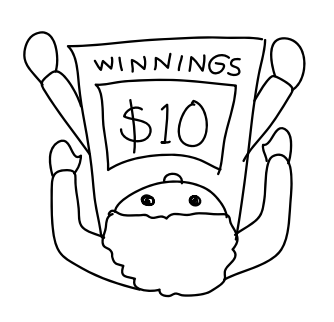
\includegraphics[scale = 0.23]{./figures/armed.png}
			\end{figure}
		\end{column}
		\begin{column}{0.8\textwidth}  %%<--- here
			\begin{figure}
				
\includegraphics[scale = 0.23]{./figures/table.png}
			\end{figure}
		\end{column}
	\end{columns}		
	
	\vspace{0.4cm}
	
	\begin{itemize}
		\item \textbf{What are Bandits}?
		\vspace{0.3cm}
		
		\begin{itemize}				
			\item Baby Reinforcement Learning.
			
			\vspace{0.3cm}
			
			\item Acting in the face of uncertainty.			
		\end{itemize}				
	\end{itemize}
\end{frame}


\begin{frame}
	\frametitle{What are Bandits?}
	
	\begin{itemize}
		\item A finite action set $\cA = \{1, \dots, k\}$
		
		\item For each $a \in \cA$, there is an \textit{unknown} distribution $\Prob_a$
		
		\item Learner chooses $A_t \in \cA$ and observes $R_t \sim \Prob_{A_t}$
		
		\item \textbf{Goal}: Maximize $\sum_{t = 1}^{n} R_t$
	\end{itemize}

	\begin{columns}
		\begin{column}{0.6\textwidth}				
		\end{column}
		\begin{column}{0.4\textwidth}  %%<--- here
			\begin{center}
				\begin{figure}
					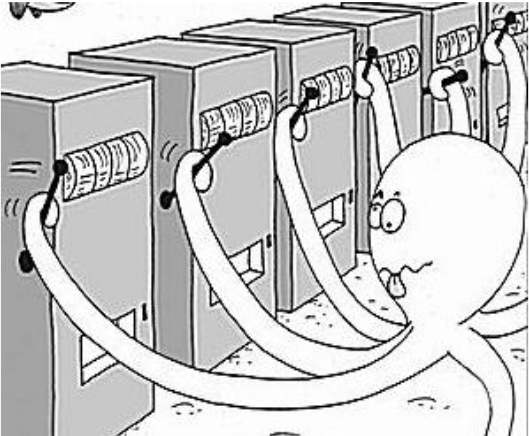
\includegraphics[scale = 0.23]{./figures/karmed.png}
				\end{figure}				
			\end{center}
		\end{column}
	\end{columns}
\end{frame}


\begin{frame}
	\frametitle{Why Bandits?}
	
	\begin{itemize}
		\item \textbf{Many applications}

		\vspace{0.5cm}		
		\begin{itemize}
			\item Clinical trials/dose discovery
			
			\item Advert placement
			
			\item Ranking (eg., for search)
			
			\item Dynamic pricing (eg., for Amazon products)
			
			\item Isolating one interesting part of reinforcement learning
		\end{itemize}
		
		\vspace{0.5cm}
		
		\item \textbf{Exploration-vs-Exploitation}

		\vspace{0.5cm}
		
		\item \textbf{Beautiful mathematics}
	\end{itemize}	
\end{frame}	



\begin{frame}
	\frametitle{Why Bandits?}
	
	\begin{itemize}
		\item Let $\mu_a$ be the \textbf{mean} of $\Prob_a$ and $\mu^\star = \max_{a\in\cA} \mu_a$.
		
		\vspace{0.3cm}
		
		\item The \textbf{optimal action} $a^\star = \arg\max_{a\in\cA} \mu_a$
		
		\vspace{0.3cm}
		
		\item The task is to minimize \textbf{Regret}: 
		\begin{equation*}
			\text{Regret}_n = n\mu^\star - \E\Big[\sum_{t = 1}^{n} R_t\Big]
		\end{equation*}
		The price paid by the learner for not knowing $\mu$.
		\vspace{0.3cm}
		
		\item To proceed, we need assumptions on the distributions:
		\begin{itemize}
			\item Bernouli
			\item Gaussian with unit variance
			\item 1-subgaussian
			\item Bounded
			\item Many more ...
		\end{itemize}
	\end{itemize}	
\end{frame}	


\begin{frame}
	\frametitle{Important Lemma}
	Let $\Delta_i = \mu^\star - \mu_i$ be the \textbf{suboptimality gap} for the \textit{i}th arm and $T_i(n)$ be the number of times arm $i$ is played over all $n$ rounds:
	\begin{block}{Lemma}
		$\text{Regret}_n = \sum_{a \in \cA} \Delta_a \E[T_a(n)]$
	\end{block}
	\textbf{Proof}:
	\begin{align*}
		\text{Regret}_n &= n\mu^\star  - \E\Big[\sum_{t = 1}^{n}R_t\Big] 
		= \E\Big[\sum_{t = 1}^{n}(\mu^\star - R_t)\Big]\\
		&= \E\Big[\sum_{t = 1}^{n}\Delta_{A_t}\Big] = \E\Big[\sum_{t = 1}^{n}\sum_{a \in \cA}\mathbf{1}(A_t = a)\Delta_{a}\Big]\\
		&= \sum_{a \in \cA}\Delta_a \E[T_a(n)],
	\end{align*}
	which concludes the proof. \qed
\end{frame}



\section{Bandit Algorithms}
\framecard{\LARGE Bandit Algorithms}

\subsection{Explore then Commit}
\begin{frame}
	\frametitle{Simplest Policy: Explore then Commit}
		\begin{algorithm*}[H]
			\SetAlgoLined
			\TitleOfAlgo{Explore then Commit}
			Choose each action $m$ times.\\
			Find the \textit{empirically} best action $I\in\{1,2,\dots,K\}$.\\
			Choose $A_t=I$ for all remaining rounds.		
		\end{algorithm*}
	
		\vspace{0.3cm}
	
		\pause
	
		\begin{alertblock}{Theorem}
			Under the 1-subgaussian assumption of reward distributions, Explore then Commit, suffers
			\vspace{-0.3cm}
			\begin{equation*}
				\text{Regret}_n \leq m\Delta + n\Delta \exp\Big(-\frac{m\Delta^2}{4}\Big).
			\end{equation*}
			\vspace{-0.3cm}
		\end{alertblock}
		\begin{itemize}
			\item 		 How to choose $m$, i.e., how much should be explore?			
			\item We have a sharp transition from explore and exploit  here. Is it possible to mix them?
		\end{itemize}


	
\end{frame}

\begin{frame}
	\frametitle{Analysis for $K = 2$}
	\vspace{0.1cm}
	\begin{itemize}
		\item Assume that $\mu_1 \geq \mu_2$.  Let $\mu_i$ be the average reward after exploring.
		\item The algorithm commits to the wrong arm if
		\begin{equation*}
		\hat\mu_2 \geq \hat\mu_1 \iff \hat\mu_2 - \mu_2 + \mu_1 - \hat\mu_1 \geq \Delta
		\end{equation*}
		\item The random variable  $\hat\mu_2 - \mu_2 + \mu_1 - \hat\mu_1$ is $\sqrt{\frac{2}{m}}$-subgaussian.
		
		\item \textbf{Regret bound}:
		\begin{align*}
		\text{Regret}_n &= \E\Big[\sum_{t= 1}^{n} \Delta_{A_t}\Big] = \E\Big[\sum_{t= 1}^{2m} \Delta_{A_t}\Big] + \E\Big[\sum_{t= 2m+1}^{n} \Delta_{A_t}\Big]\\
		&= m\Delta + (n - 2m) \Delta \Prob(\text{commit to the wrong arm})\\
		&\leq \underbrace{m\Delta}_{\text{Exploration}} + \underbrace{n\Delta \exp\big(\frac{-m\Delta^2}{4}\big)}_{\text{Exploitation}}.
		\end{align*}
	\end{itemize}
\end{frame}


\begin{frame}
	\frametitle{Analysis for $K = 2$}
	\vspace{0.1cm}
	\begin{itemize}
		\item \textbf{Regret bound}:
		$\text{Regret}_n \leq m\Delta + n\Delta \exp\big(\frac{-m\Delta^2}{4}\big)$.
		
		\vspace{0.3cm}
		
		\item Bound minimized by $m = \frac{4}{\Delta^2} \log\big(\frac{n\Delta^2}{4}\big)$:
		\begin{equation*}
			\text{Regret}_n \leq \Delta + \frac{4}{\Delta} \log\Big(\frac{n\Delta^2}{4}\Big) + \frac{4}{\Delta}.
		\end{equation*}
		\pause
		\vspace{-0.7cm}		
		\begin{columns}
			\begin{column}{0.5\textwidth}				
				\begin{figure}
					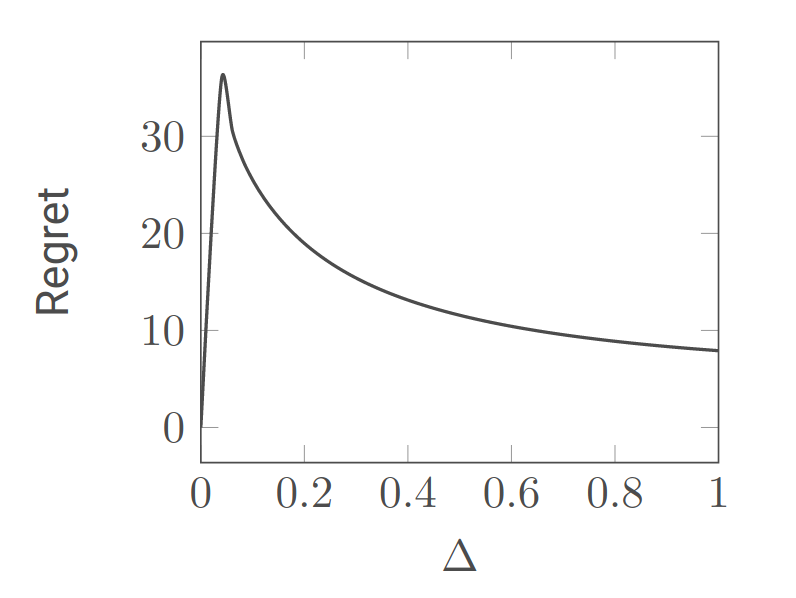
\includegraphics[scale=0.2]{./figures/regret.png}
				\end{figure}				
			\end{column}
			\begin{column}{0.55\textwidth}  %%<--- here
				\pause
				\begin{center}
					Worst case when $\Delta \approx \sqrt{\frac{1}{n}}$ with
					\begin{equation*}
						\text{Regret}_n = C \sqrt{n}.
					\end{equation*}
				\end{center}
			\end{column}
		\end{columns}

	\end{itemize}
\end{frame}

\subsection{Upper Confidence Bound}
\begin{frame}
\frametitle{Upper Confidence Bound}

	\begin{itemize}
		\item First choose an action once. 
		
		\item \textbf{Estimate}: $\hat\mu_i(t) = \frac{1}{T_i(t)} \sum_{s = 1}^{t} \mathbf{1}(A_s = i) R_s$
		
		\item Optimistic estimate of mean = largest value it could plausibly be.
		
		
				\item Choose the action maximizing:
		\begin{equation*}
		A_t  = \arg\max_{i \in \cA} \hat\mu_i(t-1) + \sqrt{\frac{2\log(t^3)}{T_i(t-1)}}
		\end{equation*}
		
		\begin{small}
			\begin{block}{Chernoff Bound}
				\vspace{0.1cm}
				If $Z_1, \dots, Z_n$ are independent $\sigma$-subgaussian, then $
				\Prob\Big(\hat\mu_n \geq \sqrt{\frac{2\sigma^2\log(1/\delta)}{n}}\Big) \leq \delta$.
				\vspace{0.04cm}
			\end{block}
		\end{small}		
		
		
		\begin{small}
			\begin{alertblock}{Regret Bound for UCB}
				Under the 1-subgaussian assumption:
				\begin{equation*}
				\Prob\Bigg(\hat\mu_n \geq \sqrt{\frac{2\sigma^2\log(1/\delta)}{n}}\Bigg) \leq \delta.
				\end{equation*}
				\vspace{-0.35cm}
			\end{alertblock}
		\end{small}
	\end{itemize}
\end{frame}

\begin{frame}
	\frametitle{Algorithmic Idea}	
	\begin{itemize}
		\item \textbf{Estimate} the mean of each arm
		\vspace{0.3cm}
		
		\item Only play arms that are statistically plausibly optimal
		\vspace{0.3cm}
		
		\item \textbf{Question}: What is this ‘statistically plausible’ and which arm to play? $\implies$ We need assumptions: Gaussian with unit variance.
		
	\end{itemize}	
\end{frame}


\end{document}